\documentclass[a4paper,11pt, twocolumn]{article}
\usepackage[margin=0.5in]{geometry}
\usepackage{graphicx}
\usepackage[font={small,it}]{caption}
\usepackage{wrapfig}
\usepackage{amsmath}
\usepackage{amssymb}
\usepackage{hyperref}

\begin{document}

\title{Comparing Classifier Methods}
\author{Alun Meredith}
\maketitle
\begin{abstract}
In this lab we sought to compare the performance of a number of different classifiers: Distance to Mean (Euclidean and Mahalanobis distances), Linear Projections (Fisher Discriminant, Random projections and mean separated), the nearest neighbour algorithm and the Bayes optimal classifier. 

To compare the performance of different machine learning classifiers it is useful to have a single value performance metric. We consider two such metrics, the first being the area under the recierver-operator characteristic (ROC) curve which refers to the probability the classifer can correctly rank two random observations with one observation from each distribution. Sometimes it was not possible or would be an extension exercise to fully evaluate the area under the ROC curve, for example the nearest neighbour algorithm. 

The second evaluation metric we will consider is the accuracy. Where applicable this was calculated from evaluating accuracy for a range of thresholds to find the greatest accuracy. The main difference between these two performance metrics is the requirement for accuracy to be at a single threshold value. This means we have to assign a cost to both false positives and false negatives to get a meaninful accuracy for each application. We will consider the case where the cost is equal but this is not always the case and it is often difficult to decide on a numerical value in such cases.

Accuracy has another weakness, if you consider a situation where the prevalence of one distribution is much smaller than the other, you are likely to get many more false positives than false negatives when trying to classify the smaller distribution. A classifier would therefore improve its accuracy simply by mindlessly classifying the larger distribution more often. To overcome this type of bias a measure called the F1 score is often used, but we will continue to use accuracy in this report as the priors are equal.

In order to compare the classifiers in a variety of situations we generated two, two dimensional normal distributions with mean $m_1$ and $m_2$ and covariance matrices $C_1$ and $C_2$. We will consider cases where the means are far apart (no overlap of distributions) and close together (strong overlap of distributions). A variety of covariance matrices were also considered, equal covariances, isotropic and non-isotropic. However unless otherwise stated I am using the default parameters, the distribution for which is shown in figure \ref{fig:distributions}:
\begin{align}
	\mathbf{m_1} = [0 \;\; 2]^t \qquad \mathbf{m_2} = [1.7 \;\; 2.5]^t \\
	\mathbf{C_1} = \mathbf{C_2} = 
	\begin{pmatrix}
	2 & 1 \\
	1 & 2
	\end{pmatrix}
\end{align}

\begin{figure}[h]
	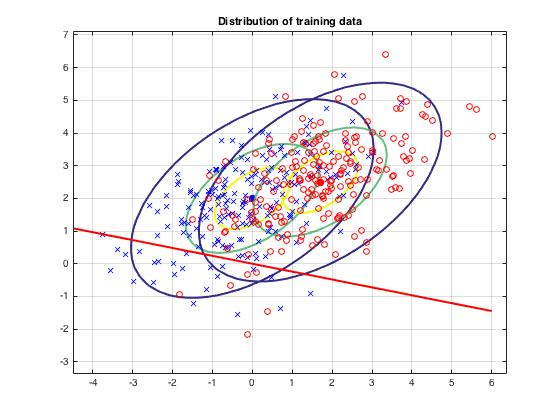
\includegraphics[width=0.7\linewidth]{trainingData.jpg}
	\centering
	\caption{Training Data of 200 samples from 2 normally distributed populations with parameters given by equation (1) and (2). Contours show lines of equal PDF for population distribution. Red line shows Fisher Linear Discriminant}
		\label{fig:distributions}
\end{figure}

\end{abstract}

\section{Linear Projections}
Any linear decision boundary between two distributions can be thought of as a threshold value boundary after the training data has been projected onto a linear vector. In lab one we discussed principal component analysis (PCA) where the data is projected onto a line to retain as much variance as possible, this preserves as much information as possible while reducing the complexity of the data. 

Although PCA is a very useful method for representing the data it is not necessarily the best way to seperate the data. In order to seperate the two distributions the main goal is to reduce the amount of overlap of the distributions after the projection. To achieve this we would like to maximise the distance between the distribution means (beetwen class scatter) while reducing the spread of the data from those means (within class scatter). To do this we maximise the ratio of the two given by the Fisher Linear Discriminant, where $\mathbf{w}$ is line on which the data is projected plus a bias term:

\begin{equation}
	J(\mathbf{w}) = \frac{|\tilde{m}_1 - \tilde{m}_2|^2}{\tilde{s}_1^2 + \tilde{s}_2^2}
\end{equation}

The line of projection is shown in figure \ref{fig:distributions} and the resultant 2 dimensional distributions shown in figure \ref{figure:projectedData}, it shows the data as quite distinguishable but with some overlap. From this point we need only pick a threshold value to have our Fisher classifier predict on future values. Note that we trained our fisher classifier on the population mean and distribution so we can use our 'training data' as a test set in this instance. 

\begin{figure}[ht]
	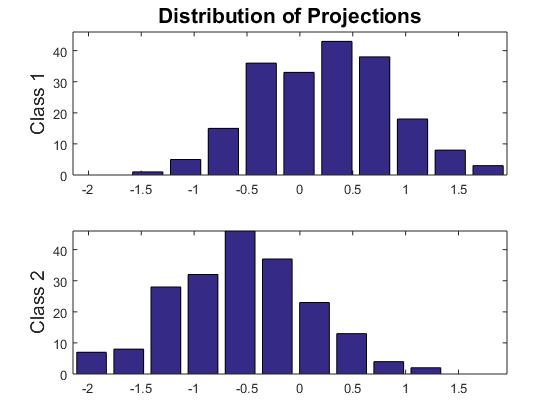
\includegraphics[width=0.7\linewidth]{ProjectionsDistribution.jpg}
	\centering
	\caption{Distribution of projected data onto fisher discriminant linear vector}
    \label{figure:projectedData}
\end{figure}

\subsection{ROC curve}
Picking a suitable threshold isn't as simple as it would seem however as type I and type II errors could have different levels of associated importance to us depending on the application. Looking at fig.\ref{figure:projectedData} we can see that if a straight line representing a threshold is drawn some values from each distribution will be incorrectly classified (on the wrong side of the line) these represent the two types of errors, falsely labelling them as class one (false positive) or missing a class one observation (false negative). In order to pick a suitable threshold frequency we plot how these error rates change as a function of the threshold chosen, known as a reciever-operator curve figure \ref{figure:ROCcurve} below:

\begin{figure}[ht]
	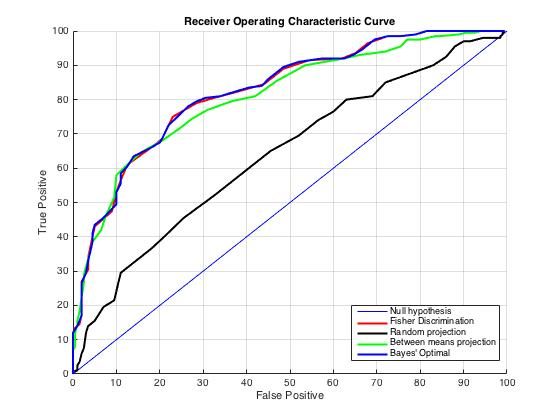
\includegraphics[width=0.7\linewidth]{ROCcurve.jpg}
	\centering
	\caption{Reciever-operator characteristic curve for different distributions}
    \label{figure:ROCcurve}
\end{figure}

The threshold is chosen subjectively as an elbow in the curve (region of relative high accuracy) around the point which represents the ratio of importance of the two errors, as stated earlier these thresholds have associated accuracies and the area under the curve represents the general ability to rank an observation from each distribution correctly. Therefore the ideal ROC curve follows the left and top borders of the graph which has an area of 1. A classifier generally speaking cannot perform worse than random (the null hypothesis) in which half the observations are correctly ranked / labelled. 

Finally our optimal Bayes' classifer is the theoretical optimal classifier assuming the data is normally distributed with equal covariances. Calculated by computing the posterior probability of one of the classes directly from the multi-dimensional gaussian equation. As shown in a previous lab this equates to a linear classifier when there is a common covariance.

\subsection{Fisher Discriminant}
We compare the effect of the fisher discriminant to these different extremes. The ROC curve gives us the impression that the fisher discriminant has approximately equal performance to the optimal Bayes' classifier for these initial conditions, certainly better than the null hypothesis or the random projection. 

Looking at the AUC for different initial conditions fig.\ref{table:AUCresults} shows that it performs roughly equivalent the the Bayes' for almost all the parameters tested with the biggest differences when the covariance matrices are unequal, which is where the ideal classifier is no longer lienar. Comparing the best accuracy of Fisher to Bayes' they are also within 1\% of eachother consistently. 

It is worth pointing out that sometimes the Fisher discriminant performs better than the Bayes' in accuracy, although this should be impossible where the Bayes' assumptions are true because the Bayes' discriminant is optimal and linear projections will always loose some information upon the projection. The results are likely the combination of the errors in the sample approximating the distribution and that the "best accuracy" is a single point averaged over 10 and therefore much more suseptable to outliers. To investigate this further we could try larger numbers of measurements, inreasing our threshold resolution and taking an average over more itterations. 

The posterior probability for Bayes' classifier is shown in figure \ref{figure:BayesDefault}. The 3d graph shows a logistic / sigmoid function when projected onto a 2d plane for the default parameters. The different values of threshold chosen simply move a linear decision boundary closer from one mean to the other at the same gradient. Because this is calculated directly from the probability density function we sampled from this form of Bayes' classifier is independent of the assumptions used to generate linear classifiers in earlier labs, but requires knowledge of the population distribution to implement. 

\begin{figure}[ht]
	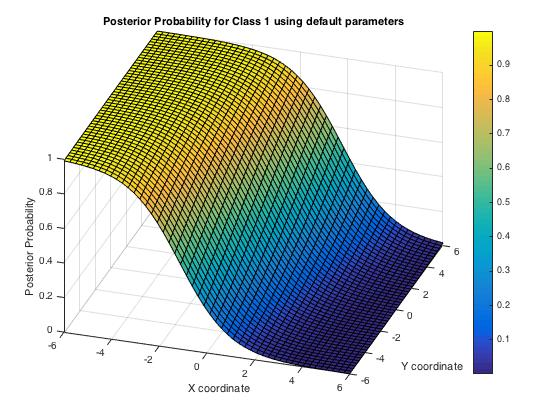
\includegraphics[width=0.7\linewidth]{3dDefault.jpg}
	\centering
	\caption{Posterior probability for default parameters}
    \label{figure:BayesDefault}
\end{figure}

When the covariances are different the quadratic terms ($\mathbf{x}^tC_i^{-1}\mathbf{x}$) which cancel for equal covariances to produce a linear order equation, no longer cancel so the resultant decision boundary will be quadratic, as shown in figure \ref{figure:BayesQuadratic}, where the decision boundary looks similar to a $\frac{1}{x^2}$ term.

\begin{figure}[ht]
	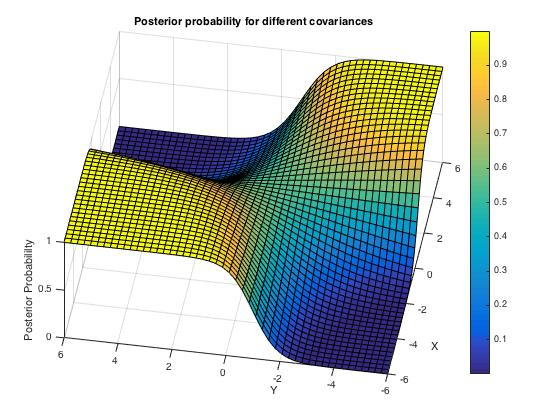
\includegraphics[width=0.7\linewidth]{3dQuadratic.jpg}
	\centering
	\caption{Posterior probability for differeing covariances}
    \label{figure:BayesQuadratic}
\end{figure}

\begin{gather}
	\mathbf{x}^tC_1^{-1}\mathbf{x} - \mathbf{x^t}C_1^{-1}\mathbf{m_1} - \mathbf{x}C_1^{-1}\mathbf{m_1^t} + \mathbf{m_1^t}C_1^{-1}\mathbf{m_1} \notag\\
	\lessgtr \\
	\mathbf{x}^tC_2^{-1}\mathbf{x}-\mathbf{x^t}C_2^{-1}\mathbf{m_2} -\mathbf{x}C_2^{-1}\mathbf{m_2^t} + \mathbf{m_2^t}C_2^{-1}\mathbf{m_2} \notag
\end{gather}
Finally the Fisher Discriminant as the optimisation of the ratio between between class and inside class scatter, it is worth considering the performance of a projection which only optimises the between class scatter. This classifier will project data onto the line which connects the means of both distributions, because in Euclidean space this seperates them furthest. We can see from the ROC curve this appears to have slightly worse performance than the Fisher discriminant or Bayes' classifier although still signifficantly better than random. This is confirmed by the accuracy and AUC were consistently marginally better with fisher. Most importantly the two classifiers performed equally well for isotropic data because in that instance the angle of projection doesn't effect the within class scatter and the biggest differences were seen for the non-isotropic unequal covariances for similar reasons. 

In summary the Fisher discriminant seems to perform very well, close or equivalent to the Bayes' optimal classifier when it is linear and still performs well when it is not. It has definite performance improvements over the means seperated linear projection. The primary reason for using the Fisher discriminant over the Bayes' classifier is the simplicity of working in one dimension, both computationally and for better comprehension. 

\section{Distance to mean classifiers}
Another method of creating linear classifiers, as seen previously was the distance to mean classifier. We saw in lab two that for isometric distributions the Bayes optimal decision boundary was simply a Euclidean distance to mean classifier. The results (table. \ref{table:AccuracyResults}) supports this as the Euclidean means classifier has equal accuracy to the Bayes' classifer for the Isotropic parameter, however for non-isotropic parameters the Euclidean distance isn't optimal. 

The Mahalanobis distance to means classifier is very similar to this except in the regard that it takes into account the covariance when computing its distance. In this sense consider the Mahalanobis distance the number of contours (shown in figure \ref{fig:distributions}) from the mean a point is. The main advantage to the Mahalanobis distance working in this way is that it can deal with non-isotropic distributions. This is shown in the results (table \ref{table:AccuracyResults}) in which the Mahalanobis classifier performed as well as the Bayes' for almost all the distribution parameters.

\section{Nearest Neighbour algorithm}

The nearest neighbour algorithm, is an algorithmic approach to producing a classifier. It follows the simple premise of assigning the new observation to the same class as the nearest training set observation to it. 

From the results (table \ref{table:AccuracyResults}) we see that the nearest neighbour algorithm performs significantly worse than the more impirical classifiers mentioned. However there are some benefits. This algorithm doesn't make any assumptions about the distributions so doesn't see significant performance drops for the non-equal covariance parameters. In addition it's accuracy can be improved by using Mahalanobis distance or considering more than one nearest neighbour. One of the selling points of nearest-neighbour is that it can be shown to have a minimum error of 2 times the error of the optimal Bayes\footnote{\url{https://en.wikipedia.org/wiki/K-nearest_neighbors_algorithm}}. This means it will continue to perform when whe assumptions which make the other classifiers we are considering work break down.

This is known as the k-nearest-neighbour algorithm, where a set of k nearest observations is taken and class assigned to the class whose mean position is closest to the new observation. In its extreme when $k \rightarrow N$ the algorithm becomes the distance to means classifer. For the K-nearest-neighbour algorithm a Kernal can be used, assigning more weight to nearer points and less to further away ones to improve the accuracy further. 

As implied by the no free lunch theorem, all of these improvements come at the cost of computational complexity. One of the biggest weakensses of the nearest neighbour algorithm is its computational complexity where each point in the training set has to be searched through for each test set point to find the nearest point.

When comparing nearest-neighbour to perceptron there are two main differences. Perceptron the way we did it is locked into producing a linear decision boundary and only really evaluates the points near the edges of the classes whereas nearest neighbour considers the whole distribution. Perceptron also had a very hard time dealing with overlapping datasets, although this can be improved by smaller learning rates it is still present. Perceptron however was much more computationally efficient and could deal with a stream of data very well as it doesn't have to recall the positions of all the previous datapoints, only the newest one and the decision boundary. 

To note is that I haven't split the data into training set and test set while testing this algorithm. Needless to say this would be an obvious extension exercise and the performance of the algorithm is likely worse than recorded. 

\begin{table}[h]
	\begin{tabular}{l*{8}{c}}
		Parameters & $C_1$ & $C_2$ & $m_1$ & $m_2$ & Fish & Rand & Means & Bayes \\
		\hline
		Default & [2 1; 1 2] & [2 1; 1 2] & $[0,2]^t$ & $[1.7,2.5]^t$ & 80.0 & 72.3 & 77.4 & 80.0 \\
		Separated & [2 1; 1 2] & [2 1; 1 2] & $[0,-3]^t$ & $[2,5]^t$ & 98.9 & 45.8 & 99.1 & 99.5 \\
		Overlapped & [2 1; 1 2] & [2 1; 1 2] & $[-1.5,2]^t$ & $[-1,2.5]^t$ &61.7 &58.0 & 61.7 & 61.7 \\
		Isotropic & [2 0; 0 2] & [2 0; 0 2] & $[0,2]^t$ & $[1.7,2.5]^t$ & 80.4 & 70.5 & 80.4 & 81.0 \\
		C1 $\neq$ C2 & 1.5 * eye(2) & 1.5 * eye(2) & $[0,2]^t$ & $[1.7,2.5]^t$ & 78.8 & 69.7 & 78.8 & 81.4 \\
		NonIso & 1.5 * eye(2) & [2 1; 1 2] & $[0,2]^t$ & $[1.7,2.5]^t$ & 81.4 & 70.2 & 80.5 & 82.7 \\
	\end{tabular}
	\caption{Area under ROC curve of different classifers for a variety of distributions averaged over 10 measurements}
	\label{table:AUCresults}
\end{table}

\begin{table}[b]
	\begin{tabular}{l*{7}{c}}
		Parameters & Fish & Rand & Means & NN & Euclid & Mahal & Bayes \\
		\hline
		Default & 73.5 & 68.8 & 71.3 & 65.1 & 71.2 & 73.1 & 73.1 \\
		Separated & 100 & 68.6 & 99.1 & 99.7 & 99.7 & 99.9 & 100 \\
		Overlapped & 60.4 & 57.8 & 60.0 & 54.1 & 58.7 & 58.7 & 58.7 \\
		Isotropic & 74.7 & 66.6 & 73.1 & 65.8 & 73.4 & 73.4 & 73.4 \\
		$C_1 \neq C_2$ & 74.7 & 67.7 & 74.3 & 66.3 & 73.4 & 72.6 & 75.0 \\
		NonIso, $C_1 \neq C_2$ & 75.4 & 67.9 & 71.8 & 66.9 & 73.9 & 74.5 & 74.4 \\
	\end{tabular}
	\caption{Best accuracy (from range of thresholds) of each classifier for a range of distributions averaged over 10 measurements}
	\label{table:AccuracyResults}
\end{table}




\end{document}
